\documentclass[a4paper,12pt]{article}
% Package to make citations superscrit with brackets
\usepackage[super,square]{natbib}
% Package to change margin size
\usepackage{anysize}
\marginsize{2cm}{2cm}{1cm}{2cm}
% Package to make headers
\usepackage{fancyhdr}
\renewcommand{\headrulewidth}{0pt}
% Package for highligths
\usepackage{soul}
% Colors for the references links
\usepackage[dvipsnames]{xcolor}
% Package to link references
\usepackage{hyperref}
\usepackage{animate}
\usepackage{graphicx}
\usepackage{float}
\hypersetup{
    colorlinks=true,
    linkcolor=black,
    citecolor=CadetBlue,
    filecolor=CadetBlue,      
    urlcolor=CadetBlue,
}
% Package for lorem ipsum
\usepackage{lipsum}
% Package for multicolumn
\usepackage{multicol}
\setlength\columnsep{18pt}
% Sets bastract
\renewenvironment{abstract}
 {\par\noindent\textbf{\abstractname} \ignorespaces:}
 {\par\noindent\medskip}

\begin{document}
\begin{center}
\Large{\textbf{Uke Tuner}}
\vspace{0.4cm}
\normalsize
\\ \textbf{Francesco Biancucci;} 984303 \\
\vspace{0.1cm}

\small{\textit{Laboratory of Making} 20/04/2023}
\medskip
\normalsize
\end{center}
{\color{gray}\hrule}
\vspace{0.4cm}
\begin{abstract}
The goal of the project was to design, program and build an automatic ukulele tuner which should be able to recognize the played note and then tune the selected string accordingly. The project was made of two main parts that needed to be designed and developed. The hardware, consisting of the circuit and the physical elements that made the motor interact with the uke and the software controlling the hardware.
\end{abstract}
{\color{gray}\hrule}
\medskip
\begin{multicols}{2}
\tableofcontents
\section{Introduction}
The project consists in a system designed to tune a ukulele without the user actively having to turn the keys. The initial idea was to create a somehow portable automatic uke tuner which uses a stepper motor to turn the uke keys in relation to the frequencies listened through a microphone. Everything needed to be controlled by an Arduino UNO R3, based on the Atmega328P chip. During the development of the project the idea shifted from a portable tuner to some sort of fixed station with four motors that needed only the uke to be put in it and then would tune the played string.\\
The final idea that was a compromise between the two because of two main reasons:
\begin{itemize}
    \item costs; using four motors makes the work easier and the project would look prettier, but the trade off between costs and the actual usefulness wasn't worth it.
    \item size; using a stepper motor such the one of choice doesn't actually save space, so the solution cannot be considered portable. Also the motor needs a decent amount of power to run, so the power supply adds to that.
\end{itemize}
\section{System Design}
When talking about the system design we should consider two different components. The circuit part, with the selection of the different components that create the final design, and the software developed to actually control the hardware.
\subsection{Circuit}
The design of the circuit went through different iterations and changed in the time, following the changes that were made because of the knowledge acquired during the development process or the necessities that needed to be satisfied to make the system work.\\
The first version of the system used a L298N H-bridge, in Fig. \ref{fig:l298n}.
\begin{figure}[H]
        \begin{center}
            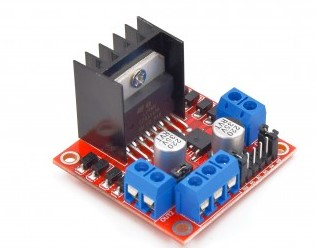
\includegraphics[width=5cm]{images/l298n.jpg}
            \caption{L298N}
            \label{fig:l298n}
        \end{center}
    \end{figure}
The L298N is a high voltage, high current dual full-bridge driver made of two integrated H-bridge inside that can support up to 46V and 2A per bridge. While with the L298N was possible to extract the source for powering the Arduino, it wasn't possible to control the output current that can go up to 2A. Such flow of current, if not handled, could damage the attached stepper motor. Moreover the dimensions of the L298N don't make it a versatile component that can be used in a circuit that doesn't take a lot of space.\\
For these reasons I decided to change from the L298N to the DRV8825 driver which allows for current flow control.
\begin{figure}[H]
    \begin{center}
        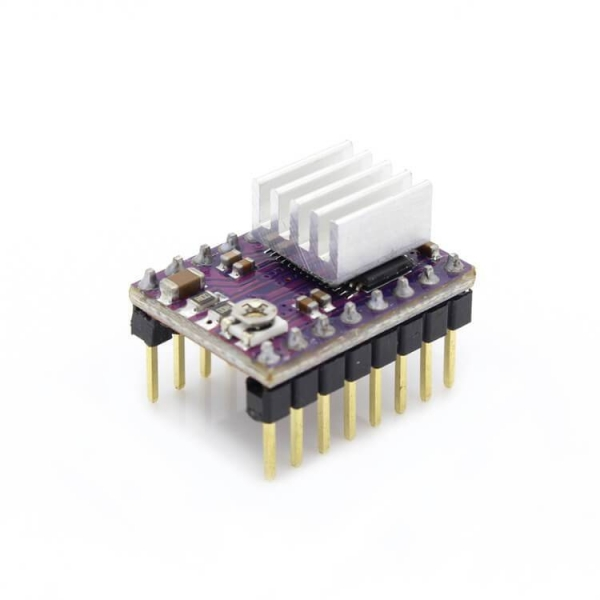
\includegraphics[width=5cm]{images/drv8825.jpg}
        \caption{DRV8825}
        \label{fig:drv8825}
    \end{center}
\end{figure}
\begin{figure}[H]
    \begin{center}
        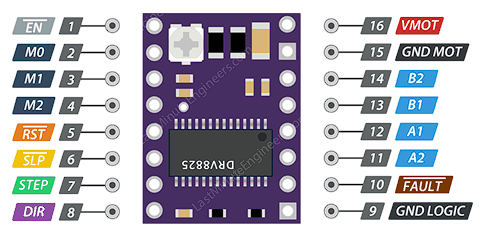
\includegraphics[width=7cm]{images/drv8825pinout.png}
        \caption{DRV8825 pinout}
        \label{fig:drv8825_pinout}
    \end{center}
\end{figure}
On a first glance it may seem an overkill but it has other useful functions that were then used inside the project. The first difference with the L298N, as said, is the ability to control the output current through an integrated resistor. The current limit is in fact determined by measuring the voltage at the ref pin (that is the resistor screw); the \textit{Vref} value should be half of the nominal current limit of the stepper.\\
By using Fig. \ref{fig:drv8825_pinout} I'll now explain the different meaning of the pins and what are the other functionalities offered by this driver.
\begin{itemize}
    \item EN is the enable pin and it is pulled LOW by default. When pulled LOW the driver is enabled, so by default the driver is enabled and can be used for a shutdown mechanism.
    \item MO, M1 and M2 are the pins used to define the step size resolution. By setting these pins to LOW/HIGH in combination is possible to control how much the stepper turns. By default these three pins are all pulled low meaning, as shown in Table \ref{tab:steps}, that the resolution is by defaul at full step. The final configuration of the driver actually used the half step to allow for better precision when turning the key.
    \item SLP is an active low pin that puts the driver to sleep when pulled LOW. It wasn't used since the tuner needs to be working almost all the time when it is powered on.
    \item RST is an active low pin too. When pulled Low the steps are ignored and it resets the driver.
    \item STEP is the controller of the microstpes of the motor. For each time it receives an HIGH pulse it drives the motor following the resolution of the microstep. E.g. if the stepper has a step of 1.8° and the resolution is full step then the motor rotates of 1.8°.
    \item DIR is the input pin that controls the direction of the motor. When pulled HIGH it turns the motor clockwise, counterclockwise when pulled LOW.
    \item VMOT e GNDMOT supply power to the motor. These pins can support a voltage between 8.2V and 45V. The module is not completely protected against voltage spikes, so as an additional protection a 100$\mu$F capacitor is put between the power supply and the pins.
    \item GND LOGIC is the ground for the logic level of the driver. It doesn't have an input logic pin since it has an internal 3V3 voltage regulator that allows the driver to drain from the motor power supply, but it needs the ground to be connected to the logic element.
    \item B2, B1, A1, A2 are the pins controlling the coils of the steppers.
    \item FAULT is a pin that when driven LOW disables the entire chip until reset or VMOT is removed. It is usually shorted to SLP.
\end{itemize}
The DRV8825 also comes with a small heatsink that helps in dissipating the heat.\\
The other elements that were changed during the development phase were the stepper itself, and I'll talk about it later, and the microphone. The first microphone used was suitable to detect audio but it wasn't able to detect the different frequencies, having only a digital output (i had this microphone already from another project). Then I switched to a microphone able to output a analog signal that could be interpreted. The problem this time around was that every sound was picked up so I ended going for the KY-037 microphone that has a reasonable precision on the analog readings and it also has a potentiometer on board that allows to adjust the threshold sensitivity.\\
\begin{figure}[H]
    \begin{center}
        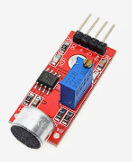
\includegraphics[width=3cm]{images/ky-037.PNG}
        \caption{ky-037}
        \label{fig:ky-037}
    \end{center}
\end{figure}
The other bits of circuitry used were two LEDs, one red and one green, used to signal if the uke string was in tune (green blink) or not (red blink). These two LEDs are connected on the 5V output line. Both LEDs have their own voltage drop and their rated current limit, from which the value of the resistances are computed. By using the Ohm's law \[V=R*I\] it is possible to get the resistances for the two LEDs.
\begin{itemize}
    \item Red led: 1.8V drop and 20mA rated current $\rightarrow$ R = (5-1.8)/0.02 = 160Ohm
    \item Green led: 2.0V drop and 20mA rated current $\rightarrow$ R = (5-2)/0.02 = 150Ohm
\end{itemize}
So i used two 200Ohm resistances.\\
The circuit also includes a LCD screen with a IIC adapter. The LCD is used to display some information during the tuning process, such as the selected string to tune or the played note when tuning. The LCD pins were soldered to the IIC adapter that allows for a smooth communication with the MCU and it also has a potentiometer on board that is used to regulate the back light of the LCD.
\begin{figure}[H]
    \begin{center}
        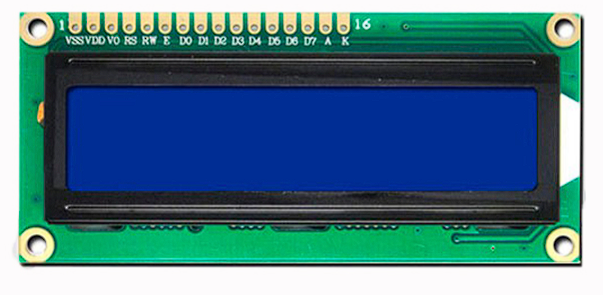
\includegraphics[width=5cm]{images/lcd1602.PNG}
        \caption{LCD}
        \label{fig:LCD}
    \end{center}
\end{figure}
To complete the circuit there is a switch that is used turn the LCD back light on and off.\\
It is reasonable to call the set of LCD and LEDs the control block of the tuner, since it is the part that allows to check the state of the tuning process. On this control block there are two more buttons and a potentiometer.\\
The first button is used to select the string to tune. After some considerations and after having studied other system used to tune guitars/ukuleles it was clear that the automatic process of recognizing the string that needs to be tuned is something that is based only on the "nearest string to the played tune" way of recognizing the string. For example if i played the G string, but the frequencies played were nearer to the A frequencies the tuner would default to tune to A. Since the system uses a motor to tune the string it was considered safer to select the string manually to avoid snapping the strings in case of a bad recognition happening.\\
The other button is used to manually turn the stepper to position the connector between the stepper and the uke key in a way that allows for connection. The potentiometer in this case is used to control the rotational speed of the motor.
\subsection{Stepper Motors}
The first used stepper motor in the project is the NEMA 17HS10-0704S that is a bipolar stepper motor with a step resolution of 1.8° and a rated current of 0.7A (Fig. \ref{fig:NEMA17HS10}. Following what has been said above the \textit{Vref} was set to 0.35A.
\begin{figure}[H]
    \begin{center}
        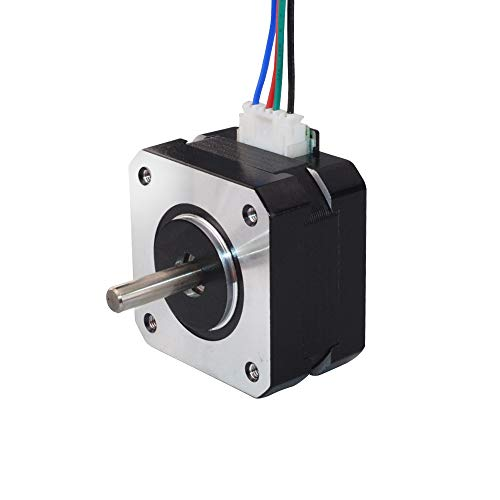
\includegraphics[width=5cm]{images/nema17-10.jpg}
        \caption{NEMA17-10}
        \label{fig:NEMA17-10}
    \end{center}
\end{figure}
As shown in the above figure the stepper has a cylindrical crankshaft that needs to be somehow connected to the uke key. There are couplers for this kind of crankshaft that can be bought but i also needed a way to connect the other end of the coupler to the key, so i decided to design my own coupler and my own connector.
\begin{figure}[H]
    \centering
    \animategraphics[autoplay, loop, width=6cm]{24}{images/coupler/goupler-}{0}{167}
    \caption{coupler}
    \label{fig:coupler}
\end{figure}
\begin{figure}[H]
    \centering
    \animategraphics[autoplay, loop, width=6cm]{24}{images/grab/grab-}{0}{82}
    \caption{grab}
    \label{fig:grab}
\end{figure}


\end{multicols}
\newpage
\section{Appendix}
\begin{figure}[H]
    \begin{center}
        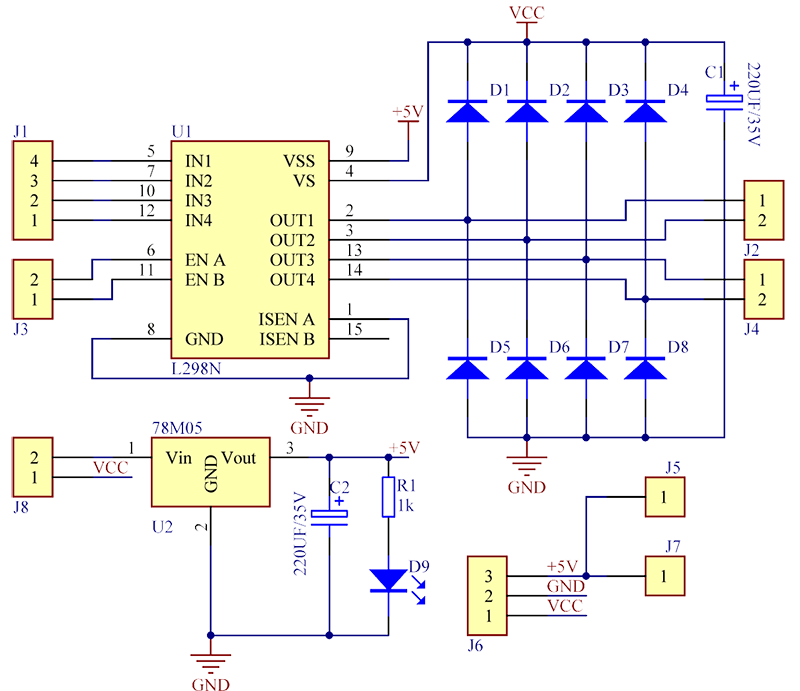
\includegraphics[width=10cm]{images/l298nschematic.png}
        \caption{L298N Schematic}
        \label{fig:l298nschematic}
    \end{center}
\end{figure}

\begin{table}[H]
\centering
\begin{tabular}{ | p{2cm}  p{2cm}  p{2cm} p{3cm}| } 
\hline
\textbf{M0} & \textbf{M1} & \textbf{M2} & \textbf{Resolution} \\
\hline
\hline
Low & Low & Low & Full Step\\
High & Low & Low & Half Step\\
Low & High & Low & 1/4 Step\\
High & High & Low & 1/8 Step\\
Low & Low & High & 1/16 Step\\
High & Low & High & 1/32 Step\\
Low & High & High & 1/32 Step\\
High & High & High & 1/32 Step\\
 \hline
\end{tabular}
\caption{Steps Resolution}
 \label{tab:steps}
 \end{table}
 \begin{figure}[H]
    \begin{center}
        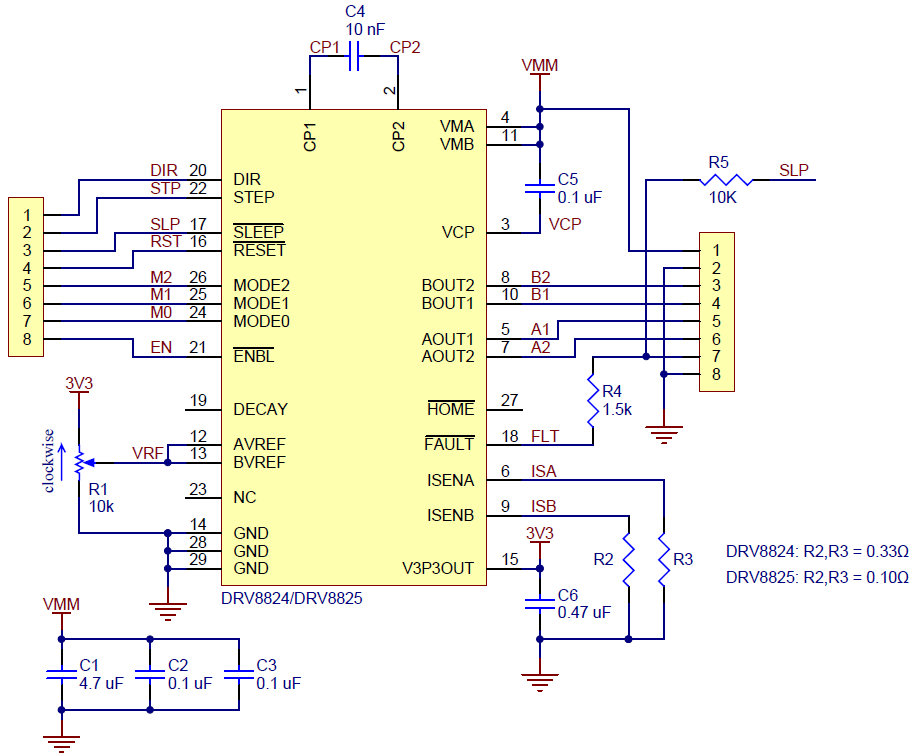
\includegraphics[width=12cm]{images/drv8825schematic.png}
        \caption{DRV8825 Schematic}
        \label{fig:drv8825schematic}
    \end{center}
\end{figure}
 \begin{figure}[H]
    \begin{center}
        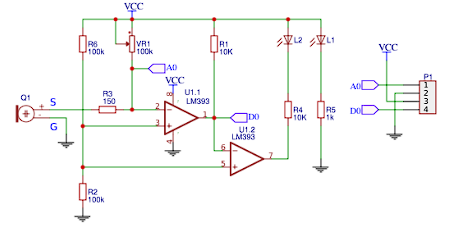
\includegraphics[width=12cm]{images/ky-037schematic.png}
        \caption{ky-037 Schematic}
        \label{fig:ky-037schematic}
    \end{center}
\end{figure}
 \begin{figure}[H]
    \begin{center}
        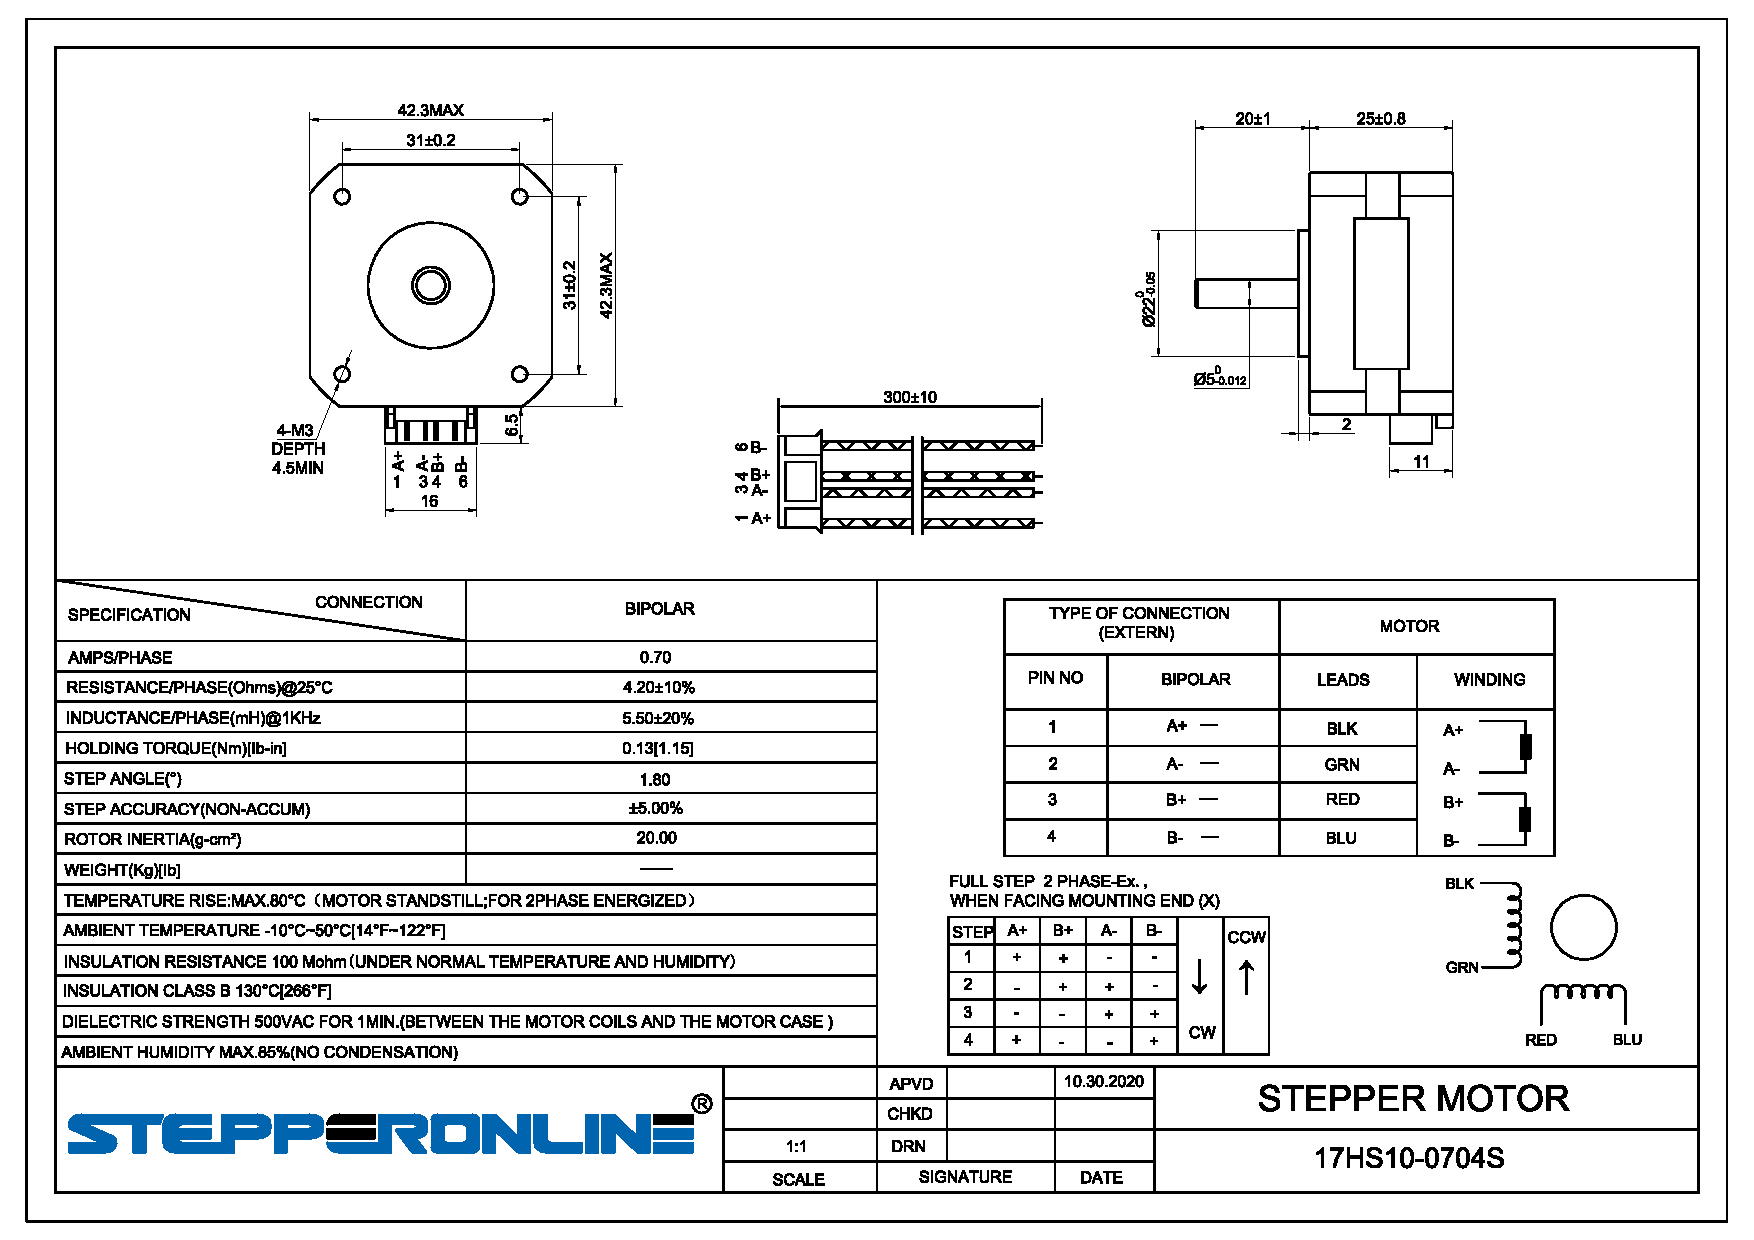
\includegraphics[width=14cm]{images/17HS10-0704S.pdf}
        \caption{NEMA17HS10 from \href{http://www.omc-stepperonline.com}{Stepperonline}}
        \label{fig:NEMA17HS10}
    \end{center}
\end{figure}
\begin{figure}[H]
    \begin{center}
        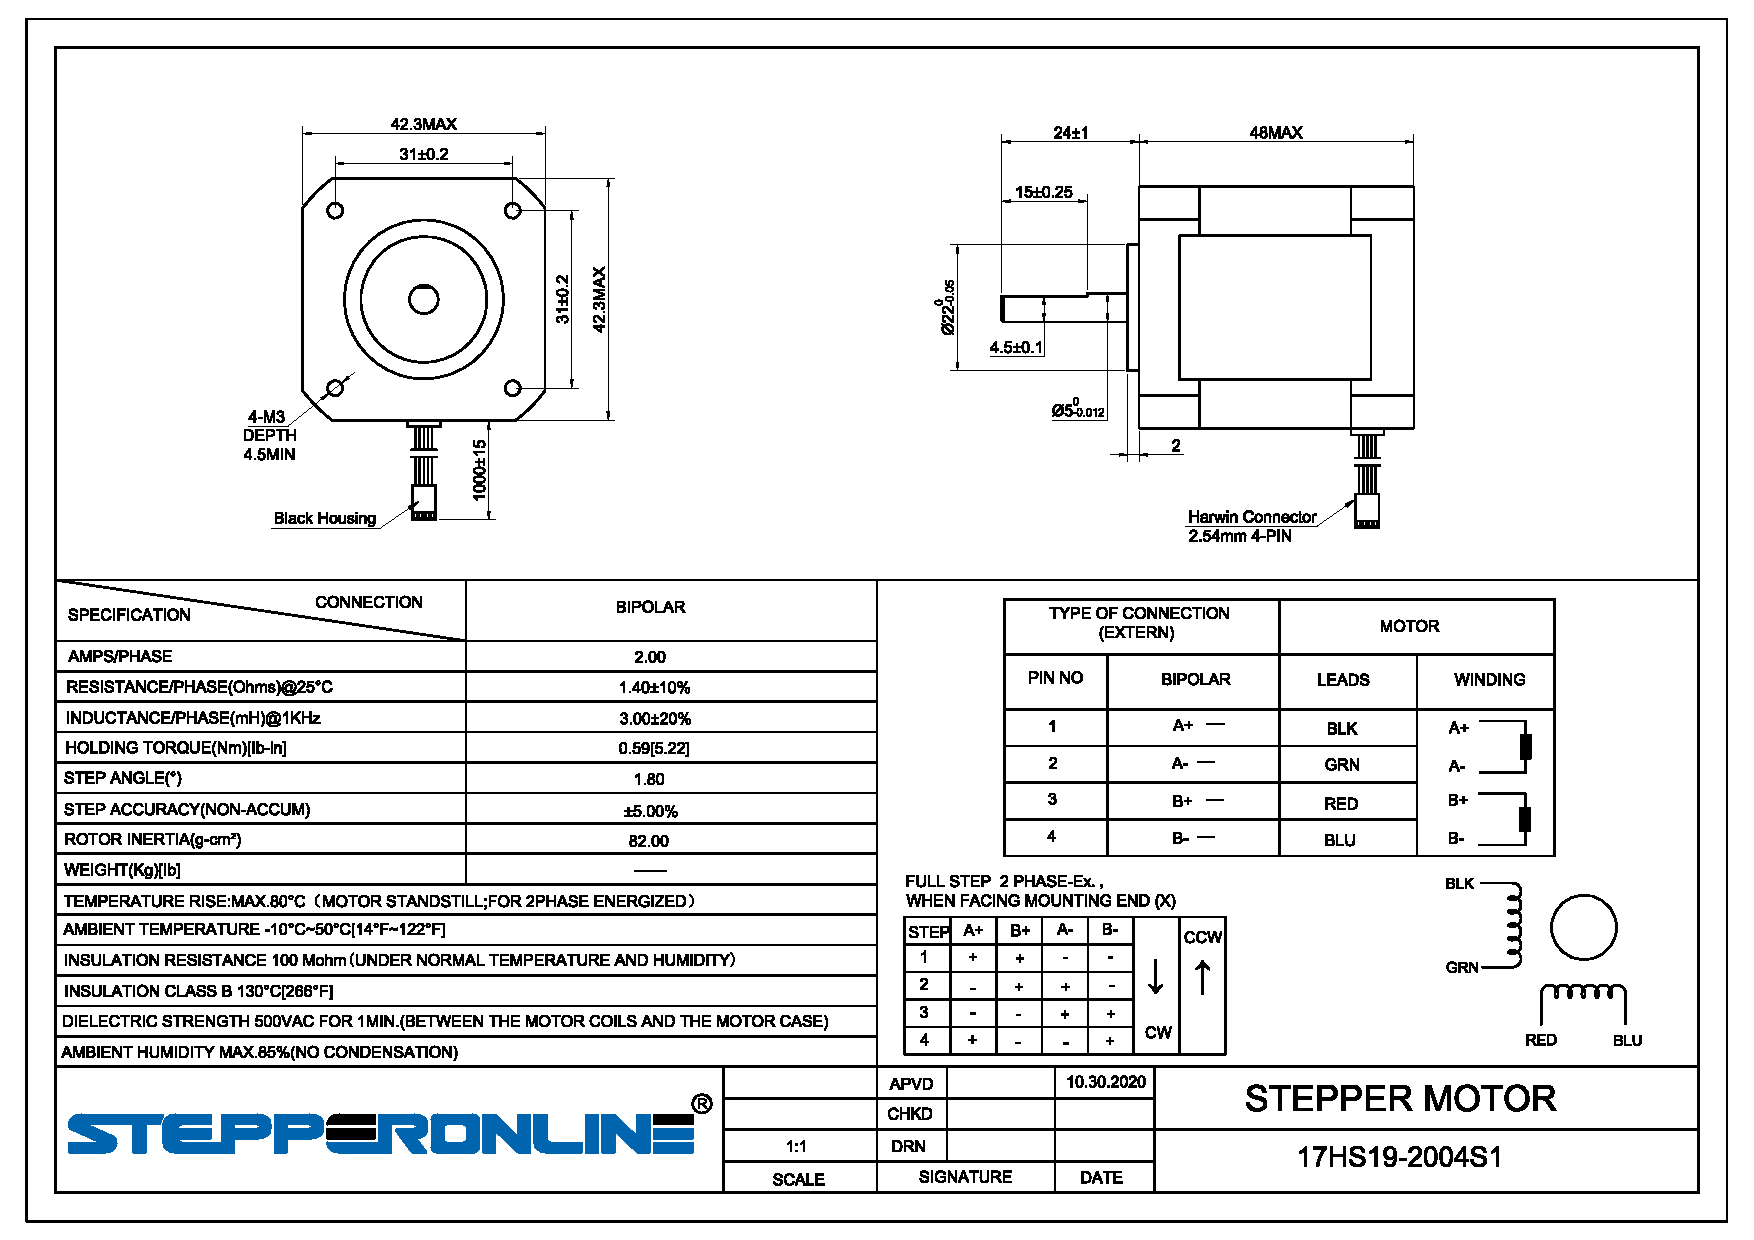
\includegraphics[width=14cm]{images/17HS19-2004S1.pdf}
        \caption{NEMA17HS19 from \href{http://www.omc-stepperonline.com}{Stepperonline}}
        \label{fig:NEMA17HS19}
    \end{center}
\end{figure}
\end{document}